\qrchapter{https://forgottenpillar.com/rsc/en-fp-chapter10}{Is God a person? - by John N. Loughborough}


\qrchapter{https://forgottenpillar.com/rsc/en-fp-chapter10}{هل الله شخص؟ - بقلم جون ن. لوبورو}


One of the earliest articles on the \emcap{personality of God} is Loughborough’s article “\textit{Is God a person?}” where he discusses the \emcap{personality of God} and His presence. It is important to remember the definition of ‘personality’ according to the Merriam-Webster dictionary: “\textit{the quality or state of being a person}”\footnote{\href{https://www.merriam-webster.com/dictionary/personality}{Merriam-Webster Dictionary - ‘\textit{personality}’}}. We will look carefully at how Loughborough sees the quality or state of God being a person.


واحدة من أقدم المقالات عن \emcap{شخصانية الله} هي مقالة لوبورو “\textit{هل الله شخص؟}” حيث يناقش \emcap{شخصانية الله} وحضوره. من المهم أن نتذكر تعريف ‘الشخصانية’ وفقًا لقاموس ميريام-ويبستر: “\textit{الصفة أو الحالة التي يكون بها الكائن شخصًا}”\footnote{\href{https://www.merriam-webster.com/dictionary/personality}{قاموس ميريام-ويبستر - ‘\textit{الشخصانية}’“}}. سننظر بعناية إلى كيف يرى لوبورو الصفة أو الحالة التي يكون بها الله شخصًا.


\begin{figure}[hp]
    \centering
    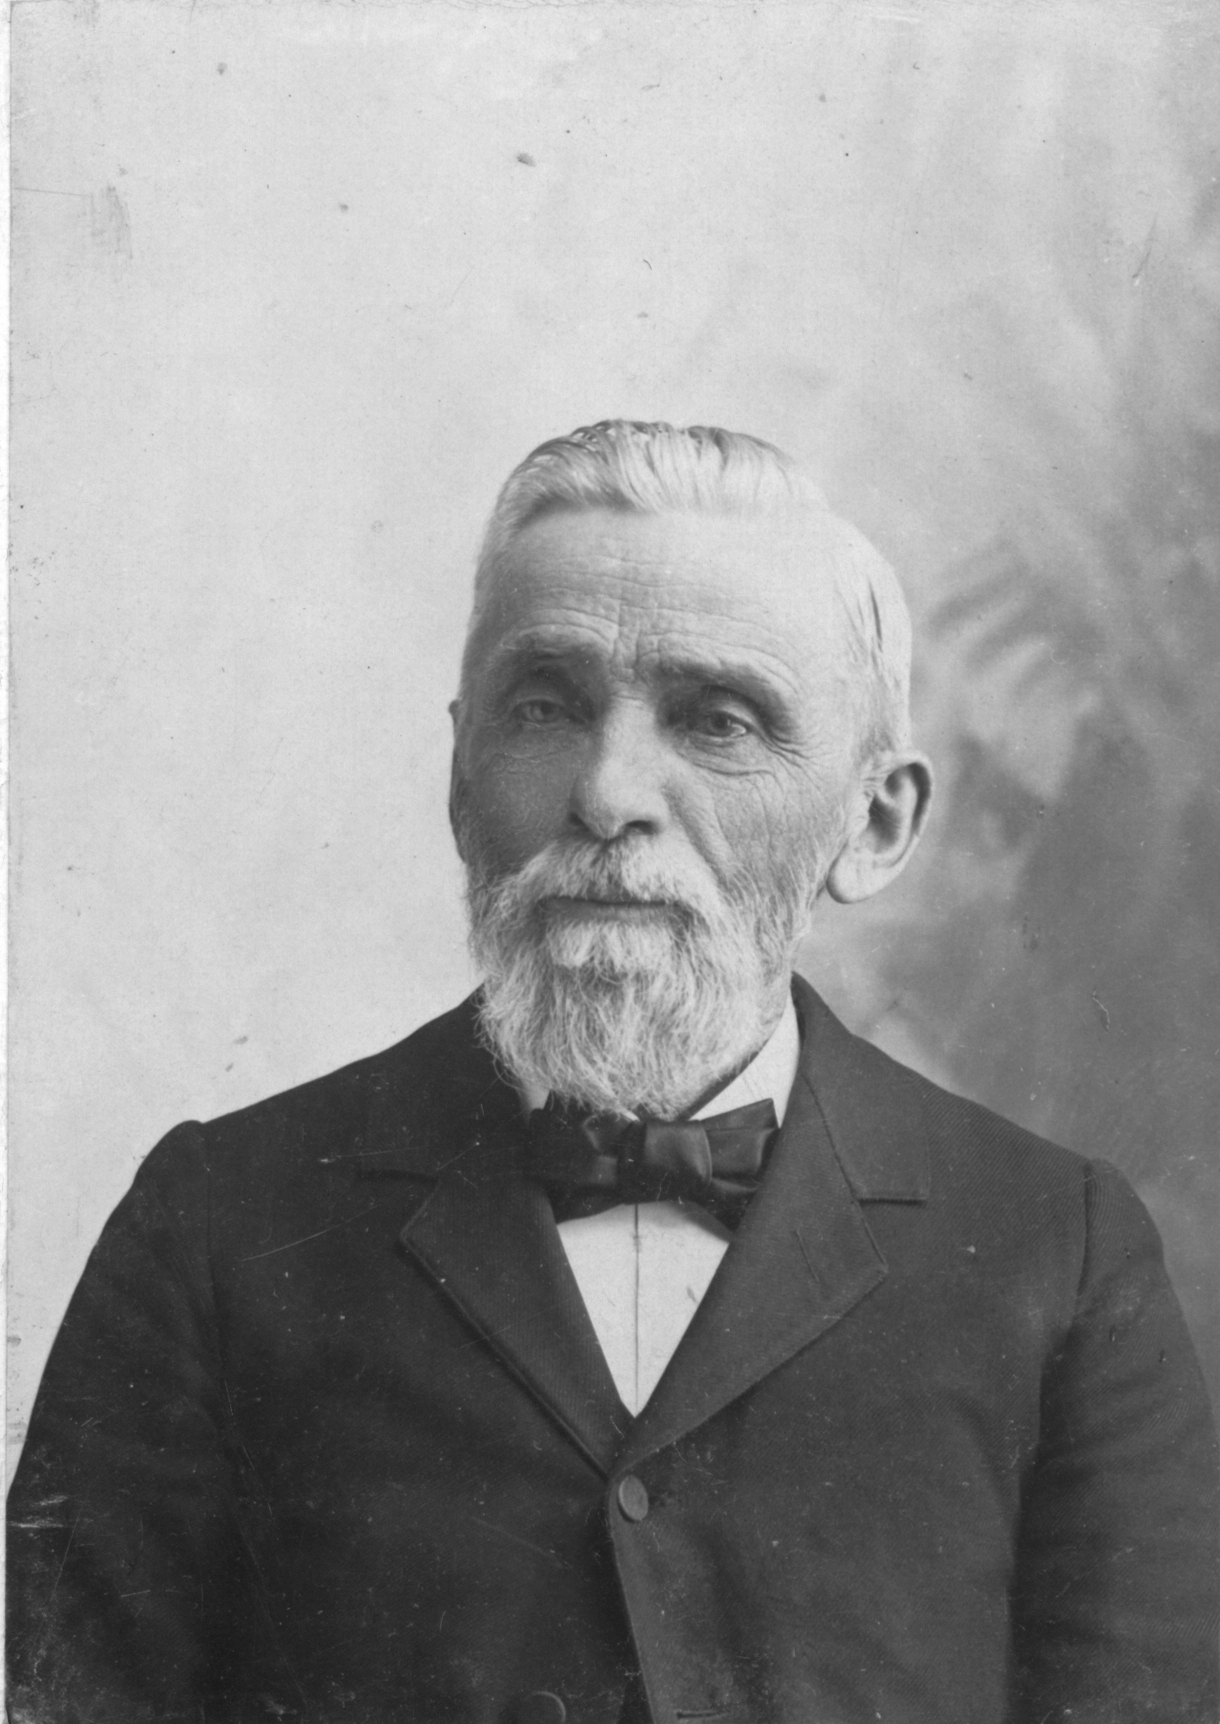
\includegraphics[width=1\linewidth]{images/john-n-loughborough.jpg}
    \caption*{John Norton Loughborough (1832-1924)}
    \label{fig:john-n-loughborough}
\end{figure}


\begin{figure}[hp]
    \centering
    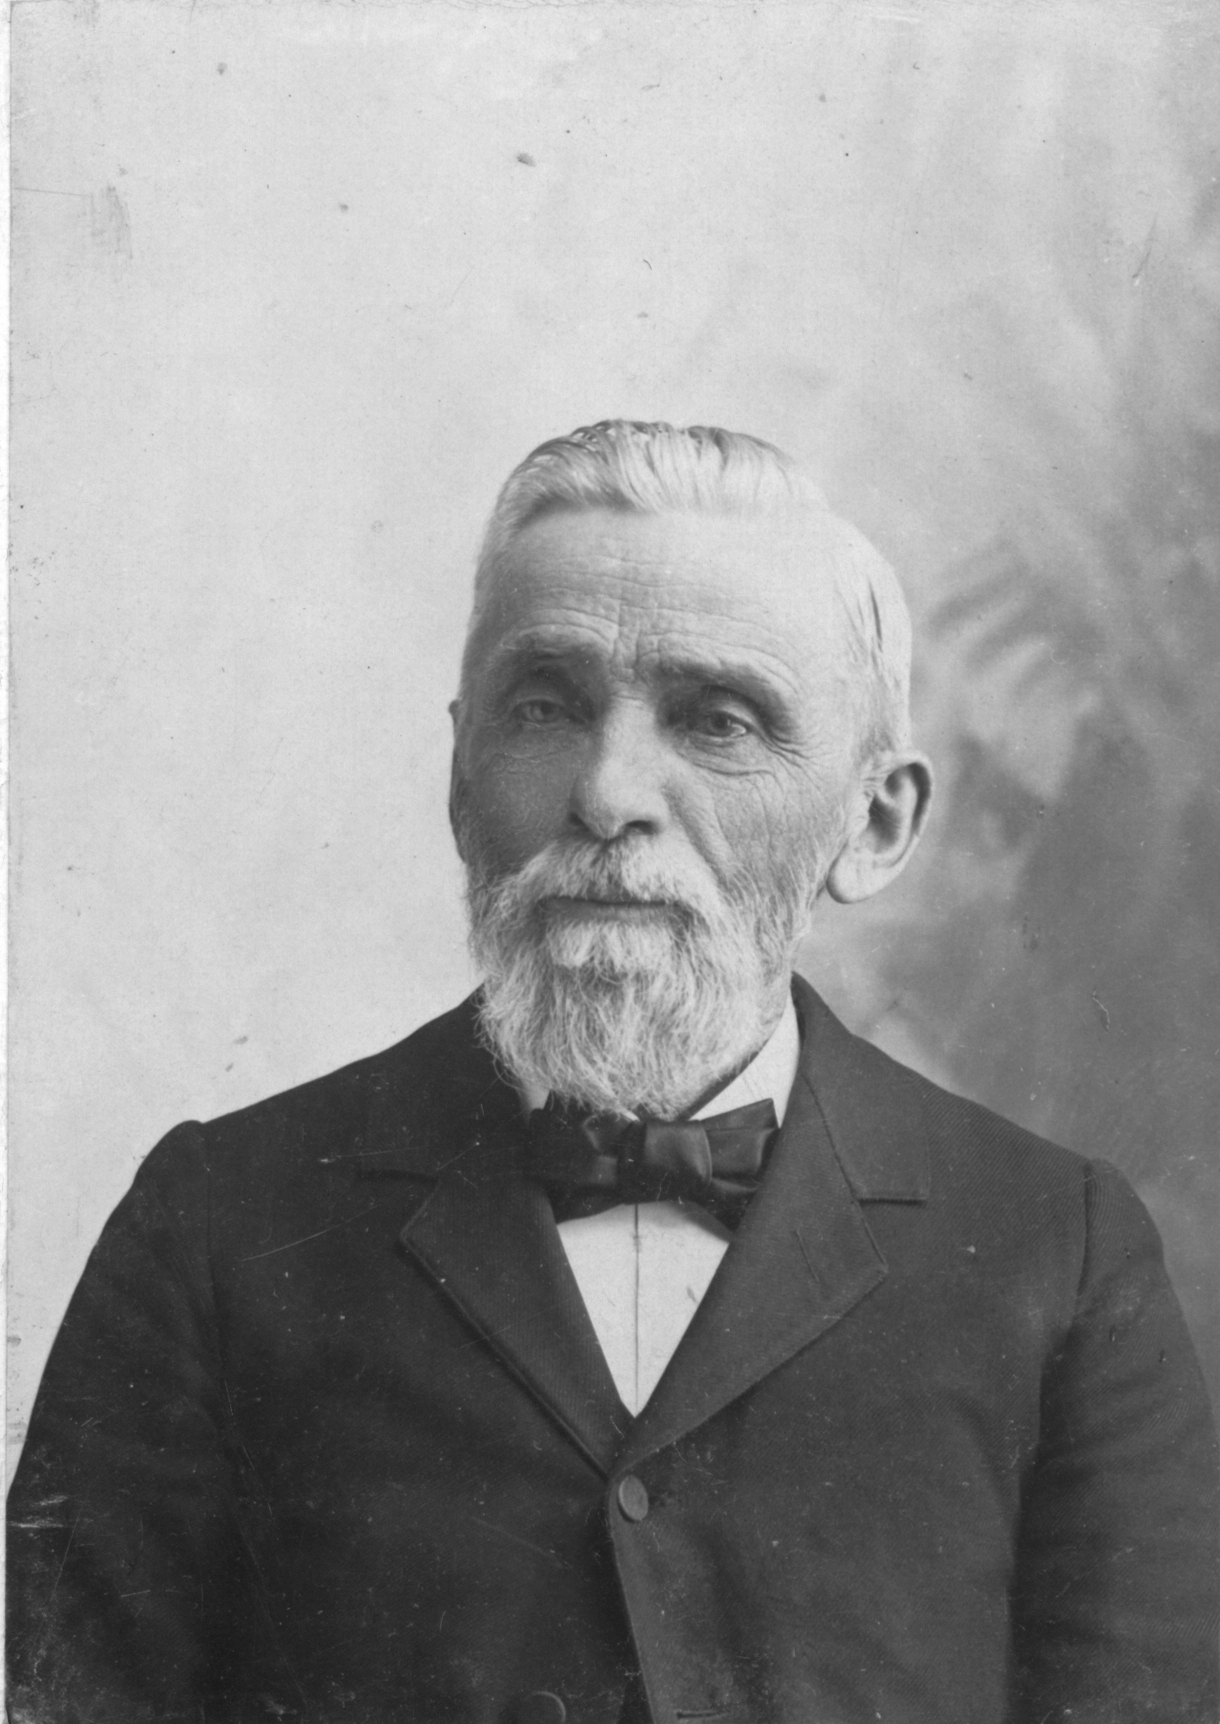
\includegraphics[width=1\linewidth]{images/john-n-loughborough.jpg}
    \caption*{جون نورتون لوبورو (1832-1924)}
    \label{fig:john-n-loughborough}
\end{figure}


\others{Whatever may be the truth in this matter, it certainly cannot be wrong for us to examine what the Word says respecting it. \textbf{Many there are that would refrain from the investigation of unpopular truths because the cry of heresy is raised against them}. We shall not consider ourselves subjects of the appellation, \textbf{neither are we prying into the secrets of the Almighty, as we pursue the investigation of this matter}. The Bible certainly contains testimony upon this point, and we again repeat, ‘\textbf{Things which are revealed belong to us}.’ We inquire then, What saith the Scripture?}


\others{مهما كانت الحقيقة في هذا الأمر، فبالتأكيد لا يمكن أن يكون من الخطأ أن نفحص ما تقوله الكلمة بخصوصه. \textbf{هناك الكثيرون الذين يمتنعون عن البحث في الحقائق غير الشائعة لأن صرخة الهرطقة تُرفع ضدها}. لن نعتبر أنفسنا موضوعًا لهذا اللقب، \textbf{ولسنا نتطفل على أسرار القدير، بينما نواصل التحقيق في هذا الأمر}. الكتاب المقدس بالتأكيد يحتوي على شهادة حول هذه النقطة، ونكرر مرة أخرى، ‘\textbf{الأمور المعلنة لنا}.’ نسأل إذن، ماذا يقول الكتاب؟}


\othersnogap{\textbf{The very testimony we have been examining in regard to man’s being formed of the dust in \underline{the image of God}, proves conclusively that \underline{God has a form}, although the sentiment is contrary to what we have been taught, while children, from the catechism}:}


\othersnogap{\textbf{إن الشهادة نفسها التي كنا ندرسها فيما يتعلق بتكوين الإنسان من التراب على \underline{صورة الله}، تثبت بشكل قاطع أن \underline{لله شكل}، على الرغم من أن هذا الرأي يتعارض مع ما تم تعليمنا إياه، ونحن أطفال، من كتاب التعليم الديني}:}


\othersnogap{Question. ‘What is God?’}


\othersnogap{سؤال. ‘ما هو الله؟‘}


\othersnogap{Answer. ‘An infinite and eternal spirit; one that always was and always will be.’}


\othersnogap{جواب. ‘روح لا نهائي وأبدي؛ واحد كان دائمًا وسيكون دائمًا.’}


\othersnogap{Q. ‘Where is God?’}


\othersnogap{س. ‘أين الله؟‘}


\othersnogap{A. ‘Everywhere.’}


\othersnogap{ج. ‘في كل مكان.’}


\othersnogap{\textbf{But we inquire, \underline{Is not God in one place more than another}?} Oh no, say you: \textbf{the Bible says \underline{he is a spirit}, and if so he must be \underline{everywhere alike}}. Well, if when man dies his spirit goes to God, it must go everywhere. \textbf{But the Bible certainly represents God as located in heaven. ‘For he hath looked down from the height of his sanctuary: from heaven did the Lord behold the earth.’ Psalm 102:19}. \textbf{Then certainly heaven cannot be everywhere, for God is represented as looking down from it. ‘\underline{Elijah went up} by a whirlwind \underline{into heaven}.’ 2 Kings 2:11}. \textbf{But, says one, does not the Bible represent God \underline{as everywhere present}?} Psalm 139:8, 9, 10. ‘If I ascend up into heaven, \textbf{thou art there}: if I make my bed in hell, \textbf{behold, thou art there}; if I take the wings of the morning, and dwell in the uttermost parts of the sea,\textbf{ even there shall thy hand lead me}, and thy right hand shall hold me.’}


\othersnogap{\textbf{لكننا نسأل، \underline{أليس الله في مكان واحد أكثر من غيره}؟} أوه لا، تقولون: \textbf{الكتاب المقدس يقول \underline{إنه روح}، وإذا كان كذلك فيجب أن يكون \underline{في كل مكان على حد سواء}}. حسنًا، إذا كانت روح الإنسان عندما يموت تذهب إلى الله، فيجب أن تذهب إلى كل مكان. \textbf{لكن الكتاب المقدس بالتأكيد يصور الله كموجود في السماء. ‘لأنه أشرف من علو قدسه. من السماء إلى الأرض نظر الرب.’ مزمور 102:19}. \textbf{إذن بالتأكيد لا يمكن أن تكون السماء في كل مكان، لأن الله يُصوَّر وهو ينظر منها. ‘\underline{صعد إيليا} في العاصفة \underline{إلى السماء}.’ 2 ملوك 2:11}. \textbf{لكن، يقول أحدهم، ألا يصور الكتاب المقدس الله \underline{كحاضر في كل مكان}؟} مزمور 139:8، 9، 10. ‘إن صعدت إلى السماوات \textbf{فأنت هناك}، وإن فرشت في الهاوية \textbf{فها أنت}. إن أخذت جناحي الصبح، وسكنت في أقاصي البحر، \textbf{فهناك أيضًا تهديني يدك} وتمسكني يمينك.’}


\othersnogap{We reply, \textbf{the subject is introduced in verse 7, as follows}: ‘\textbf{\underline{Whither shall I go from thy Spirit}?} \textbf{or whither shall I flee from \underline{thy presence}?}’ \textbf{The Spirit is \underline{God’s representative}}. \textbf{His power is manifested wherever he listeth, through the agency of his Spirit}. Christ, when giving the commission to the disciples, says, ‘Go ye into all the world, and preach the gospel to every creature, and lo! \textbf{I am with you alway, even unto the end of the world}.’ Now, no one would contend that Christ had been on the earth personally ever since the disciples commenced to fulfill this commission. \textbf{But his Spirit has been on the earth; the Comforter that he promised to send.} \textbf{So in the same manner God manifests himself \underline{by his Spirit} which is also the power through which he works}. ‘But if \textbf{the Spirit of him} that raised up Jesus from the dead dwell in you, \textbf{he that raised up Christ} from the dead shall also quicken your mortal bodies \textbf{\underline{by his Spirit} that dwelleth in you}.’ Romans 8:11. \textbf{\underline{Here is a plain distinction made between the Spirit, and God that raises the dead by that Spirit}}. \textbf{If the living God is a Spirit in the strictest sense of the term, and at the same time is in possession of a Spirit, then we have at once the novel idea of the Spirit of a Spirit, something it will take at least a Spiritualist to explain}.}[The Adventist Review and Sabbath Herald, September 18, 1855][https://documents.adventistarchives.org/Periodicals/RH/RH18550918-V07-06.pdf]


\othersnogap{نجيب، \textbf{تم تقديم الموضوع في الآية 7، كما يلي}: ‘\textbf{\underline{أين أذهب من روحك}؟} \textbf{ومن \underline{حضرتك} أين أهرب؟}’ \textbf{الروح هو \underline{ممثل الله}}. \textbf{قوته تظهر حيثما يشاء، من خلال وكالة روحه}. المسيح، عندما أعطى التكليف للتلاميذ، قال: ‘اذهبوا إلى العالم أجمع واكرزوا بالإنجيل للخليقة كلها، وها \textbf{أنا معكم كل الأيام إلى انقضاء الدهر}.’ الآن، لا أحد سيجادل بأن المسيح كان على الأرض شخصيًا منذ أن بدأ التلاميذ في تنفيذ هذا التكليف. \textbf{لكن روحه كانت على الأرض؛ المعزي الذي وعد بإرساله.} \textbf{وبنفس الطريقة يُظهر الله نفسه \underline{بروحه} التي هي أيضًا القوة التي يعمل بها}. ‘وإن كان \textbf{روح الذي} أقام يسوع من الأموات ساكنًا فيكم، \textbf{فالذي أقام المسيح} من الأموات سيحيي أجسادكم المائتة أيضًا \textbf{\underline{بروحه} الساكن فيكم}.’ رومية 8:11. \textbf{\underline{هنا تمييز واضح بين الروح والله الذي يقيم الموتى بذلك الروح}}. \textbf{إذا كان الله الحي روحًا بالمعنى الدقيق للكلمة، وفي نفس الوقت يمتلك روحًا، فلدينا على الفور فكرة جديدة عن روح الروح، شيء سيستغرق على الأقل روحانيًا لشرحه}.}[The Adventist Review and Sabbath Herald, September 18, 1855][https://documents.adventistarchives.org/Periodicals/RH/RH18550918-V07-06.pdf]


Allow us to make a short comment. We hope you recognize the specific topic being discussed here. The subject is the first point of the \emcap{Fundamental Principles} and the assertion is that God does have a form, for man is made in the image of God. Such understanding of God’s personality precludes the idea that God is everywhere present. Brother Loughborough gave the biblical reasons for God's omnipresence, together with the sentiment that “\textit{God is in one place more than another}”. God is everywhere present by His representative, the Holy Spirit, just as it is written in the first point of the \emcap{Fundamental Principles}. Further in this discussion, we will read that God is a spiritual being and possesses a tangible, material body, in contrast to the idea that He is purely a spirit.


اسمحوا لنا بتعليق قصير. نأمل أن تدركوا الموضوع المحدد الذي يتم مناقشته هنا. الموضوع هو النقطة الأولى من \emcap{المبادئ الأساسية} والتأكيد هو أن الله له شكل، لأن الإنسان مخلوق على صورة الله. مثل هذا الفهم لشخصانية الله يستبعد فكرة أن الله موجود في كل مكان. قدم الأخ لوبورو الأسباب الكتابية لوجود الله في كل مكان، إلى جانب الرأي القائل بأن “\textit{الله موجود في مكان أكثر من آخر}”. الله موجود في كل مكان من خلال ممثله، الروح القدس، كما هو مكتوب في النقطة الأولى من \emcap{المبادئ الأساسية}. سنقرأ لاحقًا في هذه المناقشة أن الله كائن روحي ويمتلك جسدًا ملموسًا وماديًا، على عكس فكرة أنه مجرد روح.


\others{There is at least one impassable difficulty in the way of \textbf{those who believe \underline{God is immaterial}, and heaven is not a literal, \underline{located place}: they are obliged to admit that \underline{Jesus is there bodily, a literal person}}; the same Jesus that was crucified, dead, and buried, was raised from the dead, \textbf{ascended up to heaven}, and is now \textbf{at the right hand of God}. \textbf{Jesus was possessed of flesh and bones after his resurrection}. Luke 24:39. ‘\textbf{Behold my hands and my feet, that it is I, myself; handle me, and see; \underline{for a spirit hath not flesh and bones as ye see me have}}.’ \textbf{If Jesus is there in heaven with a literal body of flesh and bones, may not heaven after all be a literal place, a habitation for a literal God, a literal Saviour, literal angels, and resurrected immortal saints?} \textbf{\underline{Oh no, says one, ‘God is a Spirit.’}} So Christ said to the woman of Samaria at the well. \textbf{It does not necessarily follow because God is a Spirit, \underline{that he has no body}}. In John 3:6, Christ says to Nicodemus, ‘\textbf{That which is born of the Spirit is spirit}.’ \textbf{If that which is born of the Spirit is spirit, then on the same principle, that which has a spiritual nature is spirit. God is \underline{a spirit being}, his nature is spirit, he is not of a mortal nature; }\textbf{\underline{but this does not exclude the idea of his having a body}}. David says, [Psalm 114:4,] ‘Who maketh \textbf{his angels spirits};’ yet \textbf{\underline{angels have bodies}}. Angels appeared to both Abraham and Lot, and ate with them. \textbf{We see the idea that angels are spirits, does not prove that they are not literal beings}.}


\others{هناك صعوبة واحدة على الأقل لا يمكن تجاوزها في طريق \textbf{أولئك الذين يعتقدون أن \underline{الله غير مادي}، وأن السماء ليست مكانًا \underline{حرفيًا محددًا}: فهم مضطرون للاعتراف بأن \underline{يسوع موجود هناك جسديًا، شخصًا حرفيًا}}؛ نفس يسوع الذي صُلب ومات ودُفن، قام من الأموات، \textbf{صعد إلى السماء}، وهو الآن \textbf{عن يمين الله}. \textbf{كان يسوع يمتلك لحمًا وعظامًا بعد قيامته}. لوقا 24:39. ‘\textbf{انظروا يديّ ورجليّ، إني أنا هو. جسوني وانظروا، \underline{فإن الروح ليس له لحم وعظام كما ترون لي}}.’ \textbf{إذا كان يسوع هناك في السماء بجسد حرفي من لحم وعظام، ألا يمكن أن تكون السماء بعد كل شيء مكانًا حرفيًا، مسكنًا لإله حرفي، ومخلص حرفي، وملائكة حرفية، وقديسين خالدين قائمين من الموت؟} \textbf{\underline{أوه لا، يقول أحدهم، ‘الله روح.’}} هكذا قال المسيح للمرأة السامرية عند البئر. \textbf{لا يتبع بالضرورة لأن الله روح، \underline{أنه ليس له جسد}}. في يوحنا 3:6، يقول المسيح لنيقوديموس، ‘\textbf{المولود من الروح هو روح}.’ \textbf{إذا كان المولود من الروح هو روح، فعلى نفس المبدأ، فإن الذي له طبيعة روحية هو روح. الله \underline{كائن روحي}، طبيعته روح، وهو ليس من طبيعة فانية؛ }\textbf{\underline{لكن هذا لا يستبعد فكرة أن له جسدًا}}. يقول داود، [مزمور 114:4،] ‘الصانع \textbf{ملائكته أرواحًا}؛‘ ومع ذلك \textbf{\underline{الملائكة لها أجساد}}. ظهرت الملائكة لكل من إبراهيم ولوط، وأكلت معهما. \textbf{نرى أن فكرة أن الملائكة أرواح، لا تثبت أنها ليست كائنات حرفية}.}


\othersnogap{It is inferred because the Bible says that God is a Spirit, that he is not a person. An inference should not be made the basis for an argument. Great Scripture truths are plainly stated, and it will not do for us to found a doctrine on inferences, \textbf{contrary to positive statements in the word of God}. If the Scripture states in positive \textbf{terms that God is a person, it will not answer for us to draw an inference from the text which says ‘God is a Spirit,’ \underline{that he has no body}}.}


\othersnogap{يُستنتج لأن الكتاب المقدس يقول إن الله روح، أنه ليس شخصًا. لا ينبغي أن يكون الاستنتاج أساسًا للحجة. حقائق الكتاب المقدس العظيمة مذكورة بوضوح، ولن يكون مناسبًا لنا أن نؤسس عقيدة على استنتاجات، \textbf{مخالفة للبيانات الإيجابية في كلمة الله}. إذا كان الكتاب المقدس ينص في \textbf{عبارات إيجابية على أن الله شخص، فلن يكون مناسبًا لنا أن نستنتج من النص الذي يقول ‘الله روح’، \underline{أنه ليس له جسد}}.}


\othersnogap{We will now present a few texts \textbf{which prove that God is a person}. Exodus 33:18, 23. ‘And he (Moses) said, I beseech thee shew me thy glory.’ Verse 20. ‘And he said, \textbf{Thou canst not see \underline{my face}, for there shall no man see me and live}.’ Verses 21-23. ‘And the Lord said, Behold there is a place by me, and thou shalt stand upon a rock: and it shall come to pass while my glory passeth by, that I will put thee in a cleft of the rock; and \textbf{will cover thee with \underline{my hand} while I pass by}; and I will take away \textbf{mine hand}, and thou shalt \textbf{see my \underline{back parts}}; but \textbf{\underline{my face} shall not be seen.’} \textbf{If God is \underline{an immaterial Spirit}, then Moses could not see him; for we are told a spirit cannot be seen by natural eyes}. \textbf{There would then be no propriety for God to say he would put his hand over Moses’ face while he passed by, (seemingly to prevent him from seeing his face,) for he could not see him}. Neither do we conceive how an immaterial hand could obstruct the rays of light from passing to Moses’ eyes. \textbf{But if the position be true \underline{that God is immaterial}, and cannot be seen by the natural eye, the text above is all superfluous}. \textbf{What sense is there in saying God put his hand over Moses’ face, to prevent him from seeing that which could not be seen}.}


\othersnogap{سنقدم الآن بعض النصوص \textbf{التي تثبت أن الله شخص}. خروج 33:18، 23. ‘فقال (موسى) أرني مجدك.’ الآية 20. ‘وقال، \textbf{لا تقدر أن ترى \underline{وجهي}، لأن الإنسان لا يراني ويعيش}.’ الآيات 21-23. ‘وقال الرب: هوذا عندي مكان، فتقف على الصخرة. ويكون متى اجتاز مجدي، أني أضعك في نقرة من الصخرة، \textbf{وأسترك \underline{بيدي} حتى أجتاز}؛ ثم أرفع \textbf{يدي}، فتنظر \textbf{\underline{ورائي}}؛ وأما \textbf{\underline{وجهي} فلا يُرى.’} \textbf{إذا كان الله \underline{روحًا غير مادي}، فلا يمكن لموسى أن يراه؛ لأننا أُخبرنا أن الروح لا يمكن رؤيته بالعيون الطبيعية}. \textbf{لن يكون هناك مناسبة لله أن يقول إنه سيضع يده على وجه موسى بينما يمر، (على ما يبدو لمنعه من رؤية وجهه،) لأنه لا يستطيع رؤيته}. ولا نتصور كيف يمكن ليد غير مادية أن تعيق أشعة الضوء من المرور إلى عيني موسى. \textbf{ولكن إذا كان الموقف صحيحًا \underline{أن الله غير مادي}، ولا يمكن رؤيته بالعين الطبيعية، فإن النص أعلاه كله زائد}. \textbf{ما معنى القول إن الله وضع يده على وجه موسى، لمنعه من رؤية ما لا يمكن رؤيته}.}


\othersnogap{Says one, I see we cannot harmonize the matter any other way, than that there was a literal body seen by Moses; but that was not God’s own body, \textbf{it was a body he took that he might show himself to Moses}. \textbf{Moses could form no just conceptions of God unless he assumed a form.} \textbf{So God took a body}. This throws a worse coloring on the matter than the first position; \textbf{for it charges God with deception; telling Moses he should see him, when in fact Moses according to this testimony did not see God, but another body}. A person must be given to doubt almost beyond recovery, that would attempt thus to mystify, and do away the force of this testimony.}[Ibid.][https://documents.adventistarchives.org/Periodicals/RH/RH18550918-V07-06.pdf]


\othersnogap{يقول أحدهم، أرى أننا لا نستطيع التوفيق بين الأمر بأي طريقة أخرى، سوى أن هناك جسدًا حرفيًا رآه موسى؛ لكن ذلك لم يكن جسد الله نفسه، \textbf{كان جسدًا اتخذه ليظهر نفسه لموسى}. \textbf{لا يمكن لموسى أن يكوّن تصورات عادلة عن الله إلا إذا اتخذ شكلاً.} \textbf{لذلك اتخذ الله جسدًا}. هذا يضفي لونًا أسوأ على المسألة من الموقف الأول؛ \textbf{لأنه يتهم الله بالخداع؛ يخبر موسى أنه سيراه، بينما في الواقع موسى وفقًا لهذه الشهادة لم ير الله، بل جسدًا آخر}. يجب أن يكون الشخص مستسلمًا للشك بما لا يمكن إصلاحه، الذي سيحاول هكذا تشويش وإزالة قوة هذه الشهادة.}[Ibid.][https://documents.adventistarchives.org/Periodicals/RH/RH18550918-V07-06.pdf]


Do you recognize that Brother Loughborough is tackling the sentiment that Dr. Kellogg would present in the Living Temple 48 years later? Dr. Kellogg said that it is true that God presented Himself in a\others{\textbf{\underline{particular form or place}}}[Dr. John H. Kellogg, The Living Temple, p.31.][https://archive.org/details/J.H.Kellogg.TheLivingTemple1903/page/n31/] because \others{there must be something more \textbf{tangible}, more \textbf{\underline{restricted}}, upon which to center the mind in worship}[bid, p.30][https://archive.org/details/J.H.Kellogg.TheLivingTemple1903/page/n30/], but that He is, in reality,\others{\textbf{far beyond our comprehension \underline{as are the bounds of space and time}}}[Ibid, p.33][https://archive.org/details/J.H.Kellogg.TheLivingTemple1903/page/n33/]. Brother Loughborough reasonably objected to the idea that God is only manifesting Himself to man as a definite Being, but in reality, is not what He presents Himself to be. Such a claim\others{charges God with deception}. Brother Loughborough continues with the affirmative, Biblical testimony that God is a material being.


هل تدرك أن الأخ لوبورو يتصدى للرأي الذي سيقدمه الدكتور كيلوغ في كتاب ذا ليفينغ تمبل بعد 48 عامًا؟ قال الدكتور كيلوغ إنه صحيح أن الله قدم نفسه في\others{\textbf{\underline{شكل أو مكان معين}}}[Dr. John H. Kellogg, The Living Temple, p.31.][https://archive.org/details/J.H.Kellogg.TheLivingTemple1903/page/n31/] لأنه \others{يجب أن يكون هناك شيء أكثر \textbf{ملموسية}، أكثر \textbf{\underline{تقييدًا}}، لتركيز العقل عليه في العبادة}[bid, p.30][https://archive.org/details/J.H.Kellogg.TheLivingTemple1903/page/n30/]، ولكنه في الواقع،\others{\textbf{يتجاوز فهمنا بكثير \underline{كما هي حدود الزمان والمكان}}}[Ibid, p.33][https://archive.org/details/J.H.Kellogg.TheLivingTemple1903/page/n33/]. اعترض الأخ لوبورو بشكل معقول على فكرة أن الله يظهر نفسه للإنسان فقط ككائن محدد، ولكنه في الواقع، ليس ما يقدم نفسه على أنه. مثل هذا الادعاء\others{يتهم الله بالخداع}. يواصل الأخ لوبورو بالشهادة الإيجابية والكتابية على أن الله كائن مادي.


\others{Exodus 24:9. ‘Then went up Moses and Aaron, Nadab and Abihu, and seventy of the elders of Israel: \textbf{and they saw the God of Israel}: and there was under \textbf{his feet} as it were a paved work of a sapphire stone, and as it were the body of heaven in its clearness.’ They were permitted to \textbf{see his feet}, but no \textbf{man can see his face and live}. \textbf{No \underline{mortal eye} can bear the dazzling brightness of that glory of the face of God}. It far exceeds the light of the sun. For the prophet says, ‘The light of the moon shall be as the light of the sun, and the light of the sun shall be \textbf{seven fold}, as the light of seven days, in the day that the Lord bindeth up the breach of his people, and healeth the stroke of their wound.’ Isaiah 30:26. Notwithstanding this seven-fold light that is then to shine, the prophet speaking of the scene says, ‘Then the moon shall be confounded, and the sun ashamed, when the Lord of hosts shall reign in mount Zion, and in Jerusalem, and before his ancients gloriously.’ Isaiah 24:23. The testimony of John is, [Revelation 21:23,] ‘And the city had no need of the sun, neither of the moon, to shine in it: for \textbf{the glory of God did lighten it,} and the Lamb is the light thereof.’}


\others{خروج 24:9. ‘ثم صعد موسى وهارون وناداب وأبيهو وسبعون من شيوخ إسرائيل: \textbf{ورأوا إله إسرائيل}: وكان تحت \textbf{قدميه} شبه صنعة من العقيق الأزرق الشفاف، وكذات السماء في النقاوة.’ سُمح لهم \textbf{برؤية قدميه}، لكن لا \textbf{يمكن لإنسان أن يرى وجهه ويعيش}. \textbf{لا \underline{عين فانية} تستطيع تحمل السطوع المبهر لمجد وجه الله}. فهو يفوق بكثير ضوء الشمس. لأن النبي يقول، ‘ويكون نور القمر كنور الشمس، ونور الشمس يكون \textbf{سبعة أضعاف}، كنور سبعة أيام، في يوم يجبر الرب كسر شعبه ويشفي ضرب جرحه.’ إشعياء 30:26. على الرغم من هذا النور السبعة أضعاف الذي سيضيء آنذاك، يقول النبي عن المشهد، ‘ويخجل القمر وتخزى الشمس، لأن رب الجنود قد ملك في جبل صهيون وفي أورشليم، وقدام شيوخه مجد.’ إشعياء 24:23. شهادة يوحنا هي، [رؤيا 21:23،] ‘والمدينة لا تحتاج إلى الشمس ولا إلى القمر ليضيئا فيها، لأن \textbf{مجد الله قد أنارها،} والخروف سراجها.’}


\othersnogap{\textbf{Infidels claim that there is a contradiction in the testimony of Moses, because he said, he talked with God face to face}. \textbf{We reply, there was a cloud between them}, but God told Moses, ‘\textbf{No man shall see me and live}.’ The Testimony of the New Testament is in harmony with that of the Old upon this subject. ‘Follow peace with all men, and holiness without which \textbf{no man shall see the Lord}.’ Hebrews 12:14. \textbf{Who with \underline{mortal eyes} could behold a light that far outshines seven fold the brightness of the sun?} Surely none but the holy can behold him, \textbf{none but immortal eyes} could bear that radiant glory. Although the Word says we cannot see God now and live, the promise is, that the \textbf{pure in heart shall see him}. Matthew 5:3. ‘Blessed are the pure in heart, \textbf{for they shall see God}.’ Revelation 22:4. ‘And \textbf{they shall see his face}, and his name shall be in their foreheads.’}


\othersnogap{\textbf{يدعي الملحدون أن هناك تناقضًا في شهادة موسى، لأنه قال، إنه تحدث مع الله وجهًا لوجه}. \textbf{نجيب، كان هناك سحابة بينهما}، لكن الله قال لموسى، ‘\textbf{لا يراني الإنسان ويعيش}.’ شهادة العهد الجديد متوافقة مع العهد القديم في هذا الموضوع. ‘اتبعوا السلام مع الجميع، والقداسة التي بدونها \textbf{لن يرى أحد الرب}.’ عبرانيين 12:14. \textbf{من الذي \underline{بعيون فانية} يمكنه أن يرى نورًا يفوق سطوعه سبعة أضعاف سطوع الشمس؟} بالتأكيد لا أحد سوى القديسين يمكنه رؤيته، \textbf{لا عيون خالدة} يمكنها تحمل ذلك المجد المشع. على الرغم من أن الكلمة تقول إننا لا نستطيع رؤية الله الآن ونعيش، فإن الوعد هو أن \textbf{أنقياء القلب سيرونه}. متى 5:3. ‘طوبى لأنقياء القلب، \textbf{لأنهم يعاينون الله}.’ رؤيا 22:4. ‘و\textbf{سينظرون وجهه}، واسمه سيكون على جباههم.’}


\othersnogap{Paul, [Colossians 1:15,] speaking of Christ, says, ‘Who is the image of \textbf{the invisible God}, the first born of every creature.’ Here Christ is said to be ‘\textbf{the image of the invisible God}.’ We have already shown, that\textbf{ Christ has a body composed of substance, flesh and bones; and he is said to be}, ‘\textbf{the image of the invisible God}.’ Well, says one, we admit his divine nature is in the image of God. If by his divine nature you mean the part that existed in glory with the Father before the world was, we reply, that which was in the beginning with God, (the Word,) \textbf{was made flesh, not came into flesh}, or as some state, \textbf{clothed upon with a human nature, but made flesh}. But says another, \textbf{God is said to be invisible}. \textbf{Because he is invisible now, it does not prove that he never will be seen}. The Word says, ‘The pure in heart \textbf{shall see him}’. Willing faith says, Amen.}


\othersnogap{بولس، [كولوسي 1:15،] متحدثًا عن المسيح، يقول، ‘الذي هو صورة \textbf{الله غير المنظور}، بكر كل خليقة.’ هنا يُقال إن المسيح هو ‘\textbf{صورة الله غير المنظور}.’ لقد أظهرنا بالفعل، أن \textbf{المسيح له جسد مكون من مادة، لحم وعظام؛ ويُقال إنه}، ‘\textbf{صورة الله غير المنظور}.’ حسنًا، يقول أحدهم، نحن نقر بأن طبيعته الإلهية هي على صورة الله. إذا كنت تعني بطبيعته الإلهية الجزء الذي كان موجودًا في المجد مع الآب قبل أن يكون العالم، نجيب، ذلك الذي كان في البدء مع الله، (الكلمة،) \textbf{صار جسدًا، ليس دخل في جسد}، أو كما يقول البعض، \textbf{اكتسى بطبيعة بشرية، بل صار جسدًا}. لكن يقول آخر، \textbf{يُقال إن الله غير منظور}. \textbf{لأنه غير منظور الآن، لا يثبت أنه لن يُرى أبدًا}. تقول الكلمة، ‘أنقياء القلب \textbf{سيرونه}’. الإيمان الراغب يقول، آمين.}


\othersnogap{Paul’s testimony in Philippians 2:5, 6, shows plainly what may be understood by the statement, that Christ is the image of God. ‘Let this mind be in you which was in Christ Jesus: who \textbf{being in the form of God}, thought it not robbery to \textbf{be equal with God}.’ \textbf{How can Christ be said to be in the form of God, if God has no form?} Romans 8:3. ‘God sending his own Son in the likeness of sinful flesh.’ \textbf{Christ is in the form of God, and in the form of men. This at once reveals to us the form of God}.}


\othersnogap{تظهر شهادة بولس في فيلبي 2:5، 6، بوضوح ما يمكن فهمه من البيان، أن المسيح هو صورة الله. ‘فليكن فيكم هذا الفكر الذي في المسيح يسوع أيضًا: الذي \textbf{إذ كان في صورة الله}، لم يحسب خلسة أن \textbf{يكون مساويًا لله}.’ \textbf{كيف يمكن القول إن المسيح في صورة الله، إذا كان الله ليس له صورة؟} رومية 8:3. ‘الله إذ أرسل ابنه في شبه جسد الخطية.’ \textbf{المسيح هو في صورة الله، وفي صورة البشر. هذا يكشف لنا على الفور صورة الله}.}


\othersnogap{\textbf{\underline{Daniel speaking of God, calls him the Ancient of days}}. Daniel 7:9. ‘And the Ancient of days did sit, \textbf{whose garment was white as snow}, and \textbf{the hair of his head} like the pure wool.’ \textbf{This personage is said to have a head, and hair; this certainly could not be said of him} \textbf{\underline{if he was immaterial and had no form}}. \textbf{But Paul’s testimony in \underline{Hebrews 1:3}, ought to settle every candid mind in \underline{regard to the personality of God}}. Speaking of Christ, he says, ‘Who being the brightness of his glory, \textbf{and the express image of his (the \underline{Father’s person})}.’ \textbf{Here then it is plainly stated \underline{God has a person}. Christ is the express image of it.} Then we can understand Christ where he says, ‘\textbf{He that hath seen me, hath seen the Father}.’ John 14:19. \textbf{He could not have meant, that he was his own father; for when he prayed he addressed his Father as another person who had sent him into the world}. He styled himself \textbf{the Son of God}. \textbf{Then he could not be the Father of which he was the son}. When he says, ‘He that hath seen me hath seen the Father,’ he must mean, that as \textbf{he was the express image of the Father’s person, those who saw him saw the likeness of the Father in him}.}[The Adventist Review and Sabbath Herald, September 18, 1855][https://documents.adventistarchives.org/Periodicals/RH/RH18550918-V07-06.pdf]


\othersnogap{\textbf{\underline{دانيال عندما يتحدث عن الله، يدعوه القديم الأيام}}. دانيال 7:9. ‘وجلس القديم الأيام، \textbf{ولباسه أبيض كالثلج}، و\textbf{شعر رأسه} كالصوف النقي.’ \textbf{يُقال إن هذا الشخص له رأس وشعر؛ هذا بالتأكيد لا يمكن أن يُقال عنه} \textbf{\underline{إذا كان غير مادي وليس له صورة}}. \textbf{لكن شهادة بولس في \underline{عبرانيين 1:3}، ينبغي أن تحسم كل عقل منصف في \underline{ما يتعلق بشخصانية الله}}. متحدثًا عن المسيح، يقول: ‘الذي، وهو بهاء مجده، \textbf{وصورة جوهره (أي جوهر \underline{الآب})}.’ \textbf{هنا إذن يُذكر بوضوح \underline{أن لله شخص}. المسيح هو صورة جوهره.} ثم يمكننا أن نفهم المسيح عندما يقول: ‘\textbf{الذي رآني فقد رأى الآب}.’ يوحنا 14:19. \textbf{لا يمكن أن يكون قصد أنه كان أباه نفسه؛ لأنه عندما صلى خاطب أباه كشخص آخر أرسله إلى العالم}. وصف نفسه بأنه \textbf{ابن الله}. \textbf{إذن لا يمكن أن يكون الآب الذي هو ابنه}. عندما يقول: ‘الذي رآني فقد رأى الآب’، يجب أن يقصد أنه بما \textbf{أنه كان صورة جوهر الآب، فإن أولئك الذين رأوه رأوا شبه الآب فيه}.}[The Adventist Review and Sabbath Herald, September 18, 1855][https://documents.adventistarchives.org/Periodicals/RH/RH18550918-V07-06.pdf]


It is important to pay attention to the biblical evidence that brother Loughborough points out in the testimony that God has a body. Brother Loughborough reviews several Bible passages proving that God does have a material body, but it is invisible to our mortal eyes. Sister White wrote the same when she said\egwinline{\textbf{The Father is all the fulness of the Godhead \underline{bodily}} and \textbf{is invisible to mortal sight}}[Ms21-1906.9; 1906][https://egwwritings.org/read?panels=p9754.16]. No mortal eye can see the Father, but that does not prove that God can never be seen. Jesus said: \bible{\textbf{He that hath seen me, hath seen the Father}}[John 14:19]. Jesus explained these words two chapters prior: \bible{Jesus cried and said, He that believeth on me, believeth not on me, \textbf{but on him that sent me}. And \textbf{he that seeth me seeth him that sent me}}[John 12:44-45]. Jesus did not send Himself, neither is Jesus the Father, one and the same person; but we see the Father in Christ because He is the \textit{express image of the Father's person}. (Hebrews 1:3). As Jesus is a person, possessing a body, so is the Father. Brother Loughborough continues to prove his point that God is a person, possessing form and shape, because man was created in the image of God.


من المهم الانتباه إلى الأدلة الكتابية التي يشير إليها الأخ لوبورو في الشهادة على أن الله له جسد. يستعرض الأخ لوبورو عدة مقاطع من الكتاب المقدس تثبت أن الله له جسد مادي، لكنه غير مرئي لأعيننا الفانية. كتبت الأخت وايت الشيء نفسه عندما قالت\egwinline{\textbf{الآب هو كل ملء اللاهوت \underline{جسديًا}} و\textbf{هو غير مرئي للنظر الفاني}}[Ms21-1906.9; 1906][https://egwwritings.org/read?panels=p9754.16]. لا يمكن لعين فانية أن ترى الآب، لكن هذا لا يثبت أن الله لا يمكن رؤيته أبدًا. قال يسوع: \bible{\textbf{الذي رآني فقد رأى الآب}}[يوحنا 14:19]. شرح يسوع هذه الكلمات قبل فصلين: \bible{فنادى يسوع وقال: الذي يؤمن بي، ليس يؤمن بي \textbf{بل بالذي أرسلني}. و\textbf{الذي يراني يرى الذي أرسلني}}[يوحنا 12:44-45]. يسوع لم يرسل نفسه، ولا يسوع هو الآب، شخص واحد ونفسه؛ لكننا نرى الآب في المسيح لأنه \textit{صورة جوهر الآب}. (عبرانيين 1:3). كما أن يسوع شخص، له جسد، كذلك الآب. يواصل الأخ لوبورو إثبات وجهة نظره بأن الله شخص، له شكل وهيئة، لأن الإنسان خُلق على صورة الله.


\others{But we will now return to the subject of The creation of man. \textbf{We have seen already that man’s being made in the image of God, could not refer to a moral image, for it would involve the absurdity that the lifeless clay of which man was formed, had a character like God}. \textbf{We now see the Scriptures clearly teach, that \underline{God is a person with a body and form}}. Then Genesis 1:26, may be understood to teach the fact, \textbf{that man was made in the form of God}. Other scriptures agree with this testimony. See Genesis 9:6. ‘Whoso sheddeth man’s blood, by man shall his blood be shed: \textbf{for in the image of God made he man}.’ \textbf{\underline{This testimony cannot apply to a spirit, or immaterial part of man: that which is in the image of God has blood}}. 1 Corinthians 11:7. ‘For a man indeed ought not to cover his head, \textbf{forasmuch as he is the image and glory of God}.’ James [Chap 3:9] speaking of the tongue says, ‘Therewith bless we God, even the Father; and therewith curse we men, \textbf{which are made after the similitude (likeness, resemblance – Webster) of God}.’ \textbf{The foregoing testimony settles the point, \underline{that the image of God does not refer to character but to form}}.}


\others{لكننا سنعود الآن إلى موضوع خلق الإنسان. \textbf{لقد رأينا بالفعل أن كون الإنسان مخلوقًا على صورة الله، لا يمكن أن يشير إلى صورة أخلاقية، لأن ذلك سينطوي على السخف بأن الطين الميت الذي تشكل منه الإنسان، كان له صفة مثل الله}. \textbf{نرى الآن أن الكتب المقدسة تعلم بوضوح، \underline{أن الله شخص له جسد وشكل}}. إذن يمكن فهم تكوين 1:26، لتعليم حقيقة، \textbf{أن الإنسان صُنع على شكل الله}. نصوص أخرى تتفق مع هذه الشهادة. انظر تكوين 9:6. ‘سافك دم الإنسان بالإنسان يُسفك دمه: \textbf{لأن على صورة الله عمل الإنسان}.’ \textbf{\underline{هذه الشهادة لا يمكن أن تنطبق على روح، أو جزء غير مادي من الإنسان: ذلك الذي هو على صورة الله له دم}}. 1 كورنثوس 11:7. ‘فإن الرجل لا ينبغي أن يغطي رأسه \textbf{لكونه صورة الله ومجده}.’ يعقوب [الإصحاح 3:9] متحدثًا عن اللسان يقول: ‘به نبارك الله الآب، وبه نلعن الناس \textbf{الذين قد تكونوا على شبه (مثال، تشابه - ويبستر) الله}.’ \textbf{الشهادة السابقة تحسم النقطة، \underline{أن صورة الله لا تشير إلى الصفة بل إلى الشكل}}.}


\othersnogap{Genesis 2:7. ‘\textbf{And the Lord God formed man of the dust of the ground, and breathed into his nostrils the breath of life; and man became a living soul}.’}[The Adventist Review and Sabbath Herald, September 18, 1855][https://documents.adventistarchives.org/Periodicals/RH/RH18550918-V07-06.pdf]


\othersnogap{تكوين 2:7. ‘\textbf{وجبل الرب الإله آدم ترابًا من الأرض، ونفخ في أنفه نسمة حياة. فصار آدم نفسًا حية}.’}[The Adventist Review and Sabbath Herald, September 18, 1855][https://documents.adventistarchives.org/Periodicals/RH/RH18550918-V07-06.pdf]


God formed man in His own image. God is a person, having a body, shape and form, and He formed man into His own image. From this reasoning we derive the obvious meaning of the Scriptures’ testimony about the \emcap{personality of God}. If we make false conceptions regarding God’s person, we are in danger of misunderstanding the other truths which are connected with man’s nature (mortality of the soul, the state of the dead, etc.). In his article, Brother Loughborough continues on to explain the connection between false doctrine on the immortality of the soul and wrong conceptions regarding the \emcap{personality of God}. His article in the Review and Herald from September 18, was taken from his book “\textit{An Examination of the Scripture Testimony}\footnote{\href{https://egwwritings.org/?ref=en_MPC.2&para=961.2}{John Norton Loughborough, An Examination of the Scripture Testimony, 1855}}.


شكّل الله الإنسان على صورته. الله شخص، له جسد وهيئة وشكل، وقد شكّل الإنسان على صورته. من هذا المنطق نستمد المعنى الواضح لشهادة الكتب المقدسة حول \emcap{شخصانية الله}. إذا كوّنا تصورات خاطئة بخصوص شخص الله، فنحن في خطر سوء فهم الحقائق الأخرى المرتبطة بطبيعة الإنسان (فناء النفس، حالة الموتى، إلخ). في مقالته، يواصل الأخ لوبورو شرح العلاقة بين العقيدة الخاطئة حول خلود النفس والتصورات الخاطئة المتعلقة بـ\emcap{شخصانية الله}. تم أخذ مقالته في مجلة الريفيو آند هيرالد من 18 سبتمبر، من كتابه “\textit{فحص شهادة الكتاب المقدس}\footnote{\href{https://egwwritings.org/?ref=en_MPC.2&para=961.2}{جون نورتون لوبورو، فحص شهادة الكتاب المقدس، 1855}}.


% Is God a person? - by John N. Loughborough

\begin{titledpoem}
    \stanza{
        In heaven's realm, upon His throne, \\
        God dwells in form, not spirit alone. \\
        A tangible being with shape and face, \\
        Beyond our sight in that holy place.
    }

    \stanza{    
        His glory shines too bright to see, \\
        No mortal eyes bear such majesty. \\
        Yet through His Spirit, everywhere present, \\
        His power extends, divine and pleasant.
    }

    \stanza{
        In Christ we glimpse the Father's form, \\
        The express image, perfect and warm. \\
        For we are made in God's own shape, \\
        Not just in virtue, soul, or trait.
    }

    \stanza{
        The dust was fashioned by His hand, \\
        In His own image, as He planned. \\
        A person true with body real, \\
        Not formless mist, as some appeal.
    }

    \stanza{
        The Father bodily, yet unseen by eye, \\
        Waits for the pure in heart to draw nigh.
    }
\end{titledpoem}